\documentclass[11pt,a4paper]{article}
\usepackage[utf8]{inputenc}
\usepackage[LGR,T1]{fontenc}
\usepackage[polutonikogreek,english]{babel}
\usepackage[utf8]{inputenc}
\usepackage{amsmath,amssymb,amsfonts,amsthm, bm}
\usepackage{array}
\usepackage{booktabs}
\usepackage{geometry}
\geometry{a4paper, margin=1.2in}
\usepackage{parskip}
\usepackage{graphicx} 
\usepackage{enumitem}
\usepackage[style=alphabetic,backend=biber]{biblatex}
\addbibresource{circles of apollonius bib.bib}
\usepackage{tikz}
\usepackage{booktabs}
\usepackage{longtable}

\usepackage{hyperref}
\hypersetup{
    colorlinks=true,
    linkcolor=blue,
    filecolor=magenta,      
    urlcolor=cyan,
}


\renewcommand{\O}{\mathcal{O}}
\newcommand{\OhC}{\mathcal{O}_C}
\newcommand{\OhCtilde}{\mathcal{O}_{\widetilde{C}}}
\newcommand{\gtilde}{\widetilde{g}}
\newcommand{\epsilonp}{\epsilon(p)}
\newcommand{\Pic}{\operatorname{Pic}}
\newcommand{\Hom}{\operatorname{Hom}}
\newcommand{\rank}{\operatorname{rank}}
\newcommand{\Spec}{\operatorname{Spec}}
\newcommand{\Proj}{\operatorname{Proj}}
\newcommand{\Bl}{\operatorname{Bl}}
\newcommand{\PP}{\mathbb{P}}
\newcommand{\ZZ}{\mathbb{Z}}
\newcommand{\CC}{\mathbb{C}}
\newcommand{\FF}{\mathbb{F}}




\newtheoremstyle{mytheoremstyle}{}{}{\itshape}{}{\bfseries}{.}{.5em}{}
\theoremstyle{mytheoremstyle}
\newtheorem{theorem}{Theorem}[section]
\newtheorem{proposition}[theorem]{Proposition}
\newtheorem{corollary}[theorem]{Corollary}
\newtheorem{lemma}[theorem]{Lemma}

\newtheoremstyle{mydefinitionstyle}{}{}{}{}{\bfseries}{.}{.5em}{}
\theoremstyle{mydefinitionstyle}
\newtheorem{definition}[theorem]{Definition}
\newtheorem{example}[theorem]{Example}
\newtheorem{remark}[theorem]{Remark}
\newtheorem{question}[theorem]{Question}



\newcommand{\HarrisThetaCite}[1]{[Harris '82, \S#1]} 


\begin{document}

\section{Apollonius's Problem via Singular Theta Characteristics}
\label{sec:apollonius_singular_theta}

\subsection{The Problem of Apollonius}

\newcommand{\cp}{\circ_+}
\newcommand{\cm}{\circ_-}

Let $\PP^2_{x,y,z}$ be the projective plane. A \textit{circle} is a plane conic curve that satisfies any of the following equivalent characterizations:
\begin{itemize}
    \item Having affine equation $(x-a)^2+(y-b)^2 = r^2$ or homogeneous equation $(x-az)^2+(y-bz)^2 = r^2z^2$ for $a,b,r\in \CC$;
    \item Passing through the \textit{circular points} $\circ_+ = (1:i:0)$ and $\circ_- = (1:-i:0)$.
    \item Defined by a single quadratic equation $f$ contained in the \textit{circular ideal} $(z, x^2 + y^2)$.
\end{itemize}
Let $\PP^5 = \PP H^0(\O(2))$ be the parameter space of conics in the plane. The parameter space of circles $\mathcal{C}$ is a linear subseries of this complete linear series. Since passing through the two circular points imposes two linear conditions, we see that $\mathcal{C}\cong \PP^3$. The linear series $\mathcal{C}$ is not basepoint-free, since every circle by definition passes through $\circ_+$ and $\circ_-$. By Bezout's theorem, any two circles $C\neq D$ intersect in $4$ points, which contains two other points $p,q$ aside from $\cp$ and $\cm$. In this case, $C$ is \textit{tangent} to $D$ at $p$ if $p = q$. 

\begin{center}
    \textit{Problem of Apollonius: Given $3$ general circles in the plane, how many circles are simultaneously tangent to all three?}
\end{center}

\begin{theorem}
    Given $3$ general circles in the plane, there are $8$ circles simultaneously tangent to all $3$. 
\end{theorem}

(Adapted from \href{https://en.wikipedia.org/wiki/Problem_of_Apollonius}{Wikipedia}) This classical problem was first posed by Apollonius of Perga in his lost treatise \emph{\foreignlanguage{greek}{Ἐπαφαί}} and survives only through Pappus’s 4th-century summary \cite[1]{Heath1981}\cite[2]{Pappus1893}.  In 1596 Adriaan van Roomen gave the first analytic solution via intersecting hyperbolas, though not by straightedge and compass alone \cite[3]{Romanus1596}.  François Viète shortly thereafter reconstructed a purely Euclidean solution by passing to limiting cases—degenerating a circle to a point or a line \cite[4]{Viete1646}.  Isaac Newton’s \emph{Principia} then recast the problem as determining a point from the differences of its distances to three fixed points \cite[5]{Newton1687}.

In the early nineteenth century, Joseph Diaz Gergonne exhibited an elegant straightedge-and-compass construction exploiting the involutive pairing of solution circles \cite[6]{Gergonne1814}, and Sophus Lie’s development of sphere geometry placed the problem in the broader context of transformation groups \cite[7]{Lie1897}.  René Descartes had already discovered in 1643 the curvature relation for four mutually tangent circles—now known as Descartes’ theorem—which underpins the iterative generation of the Apollonian gasket \cite[8]{Descartes1643}.  This fractal packing was famously described by Frederick Soddy in the 1930s \cite[9]{Soddy1936} and later connected to number theory through Ford’s analysis of Ford circles \cite[10]{Ford1938} and Hardy–Littlewood’s circle-method \cite[11]{HardyLittlewood1920}.

In the next paragraphs, we reprise a modern solution to the Problem of Apollonius in ***cite EH16. Fix a circle $D\in\mathcal{C}$. Let $Z_D$ be the locus in $\mathcal{C}$ consisting of circles tangent to $D$. Heuristically, a circle $C\in Z_D$ has two degrees of freedom, namely the point of tangency $p$ and the radius $r$, so we expect $Z_D$ to be two dimensional. 

\begin{proposition}
    The locus $Z_D:=\{C\in\mathcal{C}\mid C \text{ is tangent to } D\}\subseteq \PP^3$ is a quadric surface. 
\end{proposition}

\begin{proof}
    Consider the incidence correspondence $\Phi:= \{(p, C)\in D\times \mathcal{C}\mid C\text{ is tangent to }D \text{ at } p\}$. Let $\pi_1, \pi_2$ be the two projections from $\Phi$ to $D\cong \PP^1$ and $\mathcal{C}\cong \PP^3$. For $p$ different from the circular points, the preimage $\pi_1^{-1}(p)$ consists of circles $C$ tangent to $D$ at $p$. In other words, the order of vanishing $m_p(C\cdot D)$ is greater than or equal to $2$, which imposes two independent linear conditions on $C$. If $p = \cp$ or $\cm$, then the preimage consists of $C$ for which $m_p(C\cdot D)\geq 3$, but this again imposes two independent conditions on $C$ since $m_p(C\cdot D)\geq 1$ for $p = \cp$ or $\cm$ by default. Therefore, the fiber $\pi_1^{-1}(p)$ is isomorphic to $\PP^1$ for all $p \in D$. Hence, $\Phi$ is a $\PP^1$-bundle over $\PP^1$, which must be irreducible of dimension $2$. Since $\pi_2: \Phi\dashrightarrow \PP^3$ is birational onto its image, $Z_D$ is also $2$-dimensional. 

    The degree of $Z_D$ is computed as the number of points in the intersection of $Z_D$ with a general line in $\mathcal{C}$. A general line in $\mathcal{C}$ is represented by a pencil of circles on the plane. Take $2$ general circles $C_1 = Z[f], C_2=Z[g]$ which are different from $D$ and consider the pencil $\overline{C_1C_2}$. Suppose that $C_1\cap D = \{p_1, q_1\}$ and $C_2\cap D = \{p_2, q_2\}$.  The equations $f, g$ define a rational function $(f/g)|_D: D\dashrightarrow \PP^1$ which has two zeros $p_1, q_1$ and two poles $p_2, q_2$, so it extends to a double cover $D\to \PP^1$ of degree $2$ branched along $2$ points. The ramification locus of this cover contains exactly circles $C^\prime$ in the pencil that are tangent to $D$. By Riemann-Hurwitz, the size of this ramifination locus is $2$. Therefore, $Z_D$ is a quadric surface in $\mathcal{C}\cong \PP^3$. 
\end{proof}
\begin{proof}
    \textbf{\textit{Solution to the Problem of Apollonius.}} Let $D_1, D_2,$ and $D_3$ be the three given circles. After verifying transversality ***cite EH16 \S 6, it can be shown that the scheme-theoretic intersection $Z_{D_1}\cap Z_{D_2}\cap Z_{D_3}$ is zero-dimensional and consists of circles simultaneously tangent to all three given ones. The degree of this locus is $2^3 = 8$. This proves that there are $8$ circles tangent to all three general circles. 
\end{proof}

\subsection{A Naïve Approach to Monodromy}

To calculate the monodromy of the $8$ solutions, one might consider the parameter space of unordered triples of circles in the plane, and the $8:1$ cover parametrizing tuples of three circles and the eight Apollonian circles. However, it is not easy to study the geometry of these parameter spaces. We need a different approach to proceed.

\subsection{Theta Characteristics on Singular Curves}

Harris in ***cite har82 computes the monodromy of this cover using a completely different geometric construction related to theta characteristics on \textit{singular} genus 3 curves. Recall ***from sec3 that for a smooth curve $C$, a $\theta$-characteristic is a line bundle $L$ such that $L^{\otimes 2} \cong \omega_C$, where $\omega_C$ is the canonical bundle. A \textit{semicanonical divisor} $D$ is a divisor such that $2D\sim K_C$. If $C$ is non-singular, then semicanonical divisors are in one-to-one correspondence with theta characteristics. When $C$ is singular, the role of the canonical bundle is replaced by the dualizing sheaf $\omega_C^{\circ}$, but in general $\omega_C^{\circ}$ need not be locally free. The minimal setting to make sense of the definition of a theta characteristic is the Gorenstein condition. 
\begin{definition}
A reduced algebraic curve $C$ is \textbf{Gorenstein} if all its local rings $\mathcal{O}_{C,p}$ are Gorenstein local rings.
\end{definition}
From now on, let $C$ denote a projective Gorenstein curve. In this case, the set $S(C)$ of all $\theta$-characteristics on $C$ remains a principal homogeneous space for $J_2(C) = \Pic^0(C)[2]$, the group of 2-torsion line bundles on $C$. The classification of \textbf{even} ($h^0(C,L)$ is even) and \textbf{odd} ($h^0(C,L)$ is odd) theta characteristics, denoted $S^\pm(C)$ resp., carries over directly, as does the definition of the theta-form $q_L(\omega) = h^0(L \otimes \omega) - h^0(L) \pmod 2$ and its fundamental connection to the Weil pairing $\lambda$ via the Riemann-Mumford relation \HarrisThetaCite{1d}. 

\paragraph{The $2$-torsion subgroup of the Jacobian.}
To study $S(C)$, it suffices to understand the structure of $J_2(C)$ for $C$ singular. Let $\pi: \widetilde{C} \to C$ be the normalization of our reduced Gorenstein curve $C$. There is a short exact sequence of sheaves $$0\to \OhC^\times \to \pi_*\OhCtilde^\times \to \mathcal{F}\to 0,$$
where $\mathcal{F}$ is a skyscraper sheaf supported at the singular points. By the long exact sequence of sheaf cohomology, we have \begin{gather}
    0\to k^\times\to H^0(\pi_*\OhCtilde^\times)\to H^0(\mathcal{F}) \\
    \to \Pic(C) \to \Pic(\widetilde{C})\to H^1(\mathcal{F}) = 0
\end{gather}
where $H^1(\mathcal{F}) = 0$ since $\mathcal{F}$ is flasque. Let $\Gamma:=H^0(\mathcal{F})/\operatorname{im}H^0(\pi_*\OhCtilde^\times)$. There is a short exact sequence $$0\to \Gamma \to J(C)\xrightarrow{\pi^*} J(\widetilde{C})\to 0,$$
so the group $\Gamma$ consists of classes of line bundles $[L]$ for which $\pi^*L $ on $\widetilde{C}$ is trivial. Taking 2-torsion, we have a left exact sequence $$0\to \ker \pi^*\to J_2(C)\to J_2(\widetilde{C}).$$
\begin{definition}[\HarrisThetaCite{2a}]
The group $\mathbf{\Gamma_2}$ is defined as the kernel
\[ \Gamma_2 := \ker \left( \pi^*: J_2(C) \to J_2(\widetilde{C}) \right). \]
\end{definition}
Elements of $\Gamma_2$ are 2-torsion line bundles on $C$ that become trivial (isomorphic to $\OhCtilde$) when pulled back to the normalization $\widetilde{C}$. These line bundles intrinsically capture information about how $C$ is formed from $\widetilde{C}$ through identifications at its singular points. If $C$ were smooth, $\widetilde{C}=C$ and $\Gamma_2$ would be trivial.

The structure of $\Gamma_2$ is local \HarrisThetaCite{2b}. For each singular point $p \in C$ with preimages $\pi^{-1}(p) = \{q_1, \dots, q_b\} \subset \widetilde{C}$, one can define generators $e_{q_i} \in \Gamma_2$, constructed by taking the trivial bundle on $\widetilde{C}$ and introducing a "-1 twist" in the gluing data at $q_i$ relative to the other $q_j$'s over $p$. These local generators satisfy relations: $\sum_{i=1}^b e_{q_i} = 0$ for each $p$. Furthermore, if $\widetilde{C}$ is reducible, then $e_{q_i}$'s satisfy the extra relation that the sum over points on each component of $\widetilde{C}$ is zero. The sum of geometric genera of components of $\widetilde{C}$ is denoted by $\widetilde{\bm{g}}$. The rank of $\Gamma_2$ as a $\ZZ/2$-vector space is denoted by $\bm{k}$.

\paragraph{The Linear Part of the Theta-Form.}
A key result from Harris is that the theta-form $q_L$, when restricted to $\Gamma_2$, behaves very nicely:
\begin{enumerate}
    \item $\Gamma_2$ is precisely the nullspace of the Weil pairing $\lambda$ on $J_2(C)$ \HarrisThetaCite{2a, Prop 2.2}. This means for any $\omega_1, \omega_2 \in \Gamma_2$, $\lambda(\omega_1, \omega_2) = 0$.
    \item As a consequence of (1) and the Riemann-Mumford relation, $q_L|_{\Gamma_2}$ is a linear functional \HarrisThetaCite{2a, Prop 2.3}.
    \item This linear functional $q_L|_{\Gamma_2}$ is independent of the initial choice of $\theta$-characteristic $L$ \HarrisThetaCite{2a, Prop 2.4}.
\end{enumerate}
\begin{definition}[\HarrisThetaCite{2a}, Def 2.5]
The above linear functional is called the \textbf{linear part of the theta-form}, denoted $l: \Gamma_2 \to \ZZ/2$.
\end{definition}
\begin{theorem}[\HarrisThetaCite{2b}, Thm 2.12]
The linear part $l$ is determined by local properties of the singularities. Specifically, for a generator $e_q$ associated with a point $q \in \widetilde{C}$ over a singularity, $l(e_q) \equiv \text{mult}_q(D) \pmod 2$, where $D$ is the adjoint divisor on $\widetilde{C}$ defined by the conductor ideal.
\end{theorem}

\paragraph{Counting Theta Characteristics on Singular Curves.}
The counts of even and odd $\theta$-characteristics on $C$ now depend on whether $l$ is identically zero. Recall that $\gtilde$ is the sum of the geometric genera of the irreducible components of $\widetilde{C}$ and $k$ is the rank of $\Gamma_2$ as a $\mathbb{F}_2$-vector space.
\begin{proposition}[\HarrisThetaCite{2a}, Cor 2.7]
If the linear part $l \not\equiv 0$, then
\[ |S^+| = |S^-| = \frac{1}{2}|S(C)| = 2^{2\gtilde + k - 1}. \]
\end{proposition}
If the linear part $l \equiv 0$, then the values $|S^+|$ and $|S^-|$ depend on another invariant $q(C) = \sum_p \epsilonp(p) \pmod 2$, where $\epsilonp(p)$ is a local invariant of the singularity $p$ related to the adjoint divisor.
\begin{proposition}[\HarrisThetaCite{2a}, Cor 2.8] \label{prop: count theta}
If the linear part $l \equiv 0$, then
\begin{itemize}
    \item When $q(C)=0$, then $|S^+| = 2^{\gtilde+k-1}(2^{\gtilde}+1)$ and $|S^-| = 2^{\gtilde+k-1}(2^{\gtilde}-1)$.
    \item When $q(C)=1$, then $|S^+| = 2^{\gtilde+k-1}(2^{\gtilde}-1)$ and $|S^-| = 2^{\gtilde+k-1}(2^{\gtilde}+1)$.
\end{itemize}
\end{proposition}

\subsection{Application: The Circles of Apollonius}
We now use the theory of $\theta$-characteristics on singular curves to compute the monodromy of the $8$ Apollonian circles, following \HarrisThetaCite{4a}.

\newcommand{\cpm}{\circ_{\pm}}

\paragraph{From Three Circles to a Singular Genus 4 Curve $C$.} Let $C_1, C_2, C_3$ be three general circles in the plane. The union $C_\text{sum} = C_1 \cup C_2 \cup C_3$ is a degree 6 plane curve. It has triple points at $\circ_+, \circ_-$ and ordinary double points at the $3 \times 2 = 6$ pairwise intersection points of $C_1, C_2, C_3$. The partial normalization $\widetilde{C}_\text{sum}\to C_\text{sum}$ at $\circ_+$ and $\circ_-$ is a singular curve in $\mathrm{Bl}_{\circ_+,\circ_-}\PP^2$ with $6$ ordinary nodes. We can use the degree-genus formula for $\PP^2$ to calculate $$g(\widetilde{C}_\text{sum}) = \frac{(6-1)(6-2)}{2} - 6 = 4.$$ If we blow down the line $\overline{\cp\cm}$, then $\mathrm{Bl}_{\circ_+,\circ_-}\PP^2$ is mapped to $\PP^1\times \PP^1$, which can be embedded in $\PP^3$ as a quadric surface $Q$. Let $\cpm$ denote the image of the line $\overline{\cp\cm}$ and let $\hat{C}_\text{sum}$ be the image of $\widetilde{C}_\text{sum}$. Then, $\Hat{C}_\text{sum}$ is a singular genus $4$ curve embedded in $\PP^3$ as a type $(2,3)$-complete intersection, so it is a canonical curve. As a result, the hyperplane sections of $Q$ are proper transforms of circles in $\PP^2$, and the original plane $\PP^2$ is related to $Q$ by projecting from the point $\cpm$. 

\begin{figure}[ht]
    \centering

\tikzset{every picture/.style={line width=0.75pt}} %set default line width to 0.75pt        

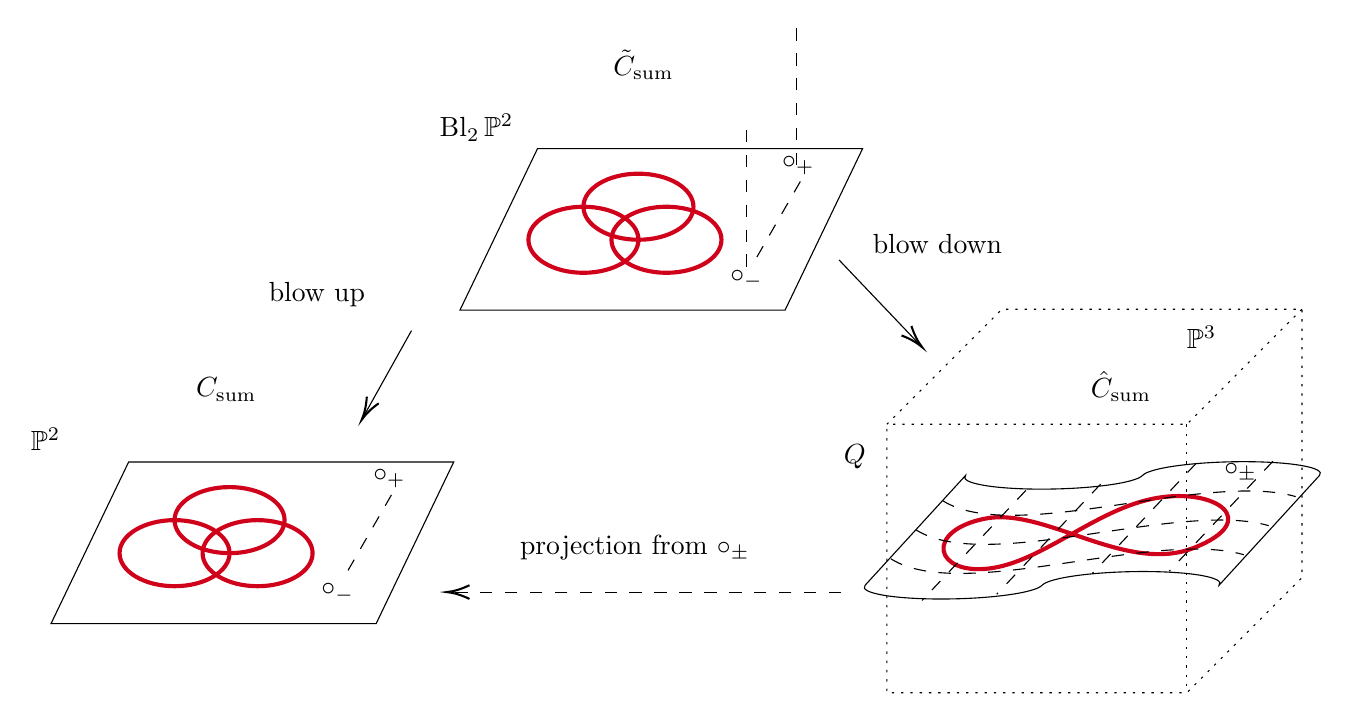
\begin{tikzpicture}[x=0.75pt,y=0.75pt,yscale=-1,xscale=1]
%uncomment if require: \path (0,359); %set diagram left start at 0, and has height of 359

%Shape: Parallelogram [id:dp5168534914761163] 
\draw   (96.7,225.17) -- (253.33,225.17) -- (215.97,303) -- (59.33,303) -- cycle ;
%Shape: Ellipse [id:dp07065059940791807] 
\draw  [color={rgb, 255:red, 208; green, 2; blue, 27 }  ,draw opacity=1 ][line width=1.5]  (118.83,253.17) .. controls (118.83,244.38) and (130.7,237.25) .. (145.33,237.25) .. controls (159.97,237.25) and (171.83,244.38) .. (171.83,253.17) .. controls (171.83,261.96) and (159.97,269.08) .. (145.33,269.08) .. controls (130.7,269.08) and (118.83,261.96) .. (118.83,253.17) -- cycle ;
%Shape: Ellipse [id:dp5379791330764142] 
\draw  [color={rgb, 255:red, 208; green, 2; blue, 27 }  ,draw opacity=1 ][line width=1.5]  (92.33,269.08) .. controls (92.33,260.29) and (104.2,253.17) .. (118.83,253.17) .. controls (133.47,253.17) and (145.33,260.29) .. (145.33,269.08) .. controls (145.33,277.87) and (133.47,285) .. (118.83,285) .. controls (104.2,285) and (92.33,277.87) .. (92.33,269.08) -- cycle ;
%Shape: Ellipse [id:dp6420045249063676] 
\draw  [color={rgb, 255:red, 208; green, 2; blue, 27 }  ,draw opacity=1 ][line width=1.5]  (132.33,269.08) .. controls (132.33,260.29) and (144.2,253.17) .. (158.83,253.17) .. controls (173.47,253.17) and (185.33,260.29) .. (185.33,269.08) .. controls (185.33,277.87) and (173.47,285) .. (158.83,285) .. controls (144.2,285) and (132.33,277.87) .. (132.33,269.08) -- cycle ;
%Straight Lines [id:da9959827347884407] 
\draw  [dash pattern={on 4.5pt off 4.5pt}]  (223.33,241) -- (200.33,281) ;
%Shape: Parallelogram [id:dp5023772298762389] 
\draw   (293.7,74.17) -- (450.33,74.17) -- (412.97,152) -- (256.33,152) -- cycle ;
%Shape: Ellipse [id:dp8810292997307249] 
\draw  [color={rgb, 255:red, 208; green, 2; blue, 27 }  ,draw opacity=1 ][line width=1.5]  (315.83,102.17) .. controls (315.83,93.38) and (327.7,86.25) .. (342.33,86.25) .. controls (356.97,86.25) and (368.83,93.38) .. (368.83,102.17) .. controls (368.83,110.96) and (356.97,118.08) .. (342.33,118.08) .. controls (327.7,118.08) and (315.83,110.96) .. (315.83,102.17) -- cycle ;
%Shape: Ellipse [id:dp6996192718122992] 
\draw  [color={rgb, 255:red, 208; green, 2; blue, 27 }  ,draw opacity=1 ][line width=1.5]  (289.33,118.08) .. controls (289.33,109.29) and (301.2,102.17) .. (315.83,102.17) .. controls (330.47,102.17) and (342.33,109.29) .. (342.33,118.08) .. controls (342.33,126.87) and (330.47,134) .. (315.83,134) .. controls (301.2,134) and (289.33,126.87) .. (289.33,118.08) -- cycle ;
%Shape: Ellipse [id:dp6219054226021791] 
\draw  [color={rgb, 255:red, 208; green, 2; blue, 27 }  ,draw opacity=1 ][line width=1.5]  (329.33,118.08) .. controls (329.33,109.29) and (341.2,102.17) .. (355.83,102.17) .. controls (370.47,102.17) and (382.33,109.29) .. (382.33,118.08) .. controls (382.33,126.87) and (370.47,134) .. (355.83,134) .. controls (341.2,134) and (329.33,126.87) .. (329.33,118.08) -- cycle ;
%Straight Lines [id:da3134822232810205] 
\draw  [dash pattern={on 4.5pt off 4.5pt}]  (420.33,90) -- (397.33,130) ;
%Straight Lines [id:da6640320946042989] 
\draw  [dash pattern={on 4.5pt off 4.5pt}]  (394.33,65.17) -- (394.33,132.17) ;
%Straight Lines [id:da02668078552186215] 
\draw  [dash pattern={on 4.5pt off 4.5pt}]  (418.33,16.17) -- (418.33,83.17) ;
%Shape: Cube [id:dp9631266037455462] 
\draw  [dash pattern={on 0.84pt off 2.51pt}] (462,206.99) -- (517.43,151.55) -- (662,151.55) -- (662,280.9) -- (606.57,336.33) -- (462,336.33) -- cycle ; \draw  [dash pattern={on 0.84pt off 2.51pt}] (662,151.55) -- (606.57,206.99) -- (462,206.99) ; \draw  [dash pattern={on 0.84pt off 2.51pt}] (606.57,206.99) -- (606.57,336.33) ;
%Flowchart: Punched Tape [id:dp5931599322049743] 
\draw   (622.05,284.55) .. controls (625.4,280.9) and (609.02,277.93) .. (585.47,277.93) .. controls (561.93,277.93) and (540.13,280.9) .. (536.79,284.55) .. controls (533.45,288.2) and (511.65,291.17) .. (488.11,291.17) .. controls (464.56,291.17) and (448.19,288.2) .. (451.53,284.55) -- (499.95,231.62) .. controls (496.6,235.27) and (512.98,238.23) .. (536.53,238.23) .. controls (560.07,238.23) and (581.87,235.27) .. (585.21,231.62) .. controls (588.55,227.96) and (610.35,225) .. (633.89,225) .. controls (657.44,225) and (673.81,227.96) .. (670.47,231.62) -- cycle ;
%Shape: Polygon Curved [id:ds011948521705470894] 
\draw  [color={rgb, 255:red, 208; green, 2; blue, 27 }  ,draw opacity=1 ][line width=1.5]  (610,266.5) .. controls (643,253.5) and (621,237.5) .. (592,242.5) .. controls (563,247.5) and (537,273.5) .. (511,276.5) .. controls (485,279.5) and (480,258.5) .. (509,252.5) .. controls (538,246.5) and (577,279.5) .. (610,266.5) -- cycle ;
%Curve Lines [id:da7065731269444068] 
\draw  [dash pattern={on 4.5pt off 4.5pt}]  (489,243.83) .. controls (523,265.33) and (616,229.33) .. (659,241.83) ;
%Curve Lines [id:da7278007658113601] 
\draw  [dash pattern={on 4.5pt off 4.5pt}]  (476,257.83) .. controls (510,279.33) and (603,243.33) .. (646,255.83) ;
%Curve Lines [id:da21951531552569103] 
\draw  [dash pattern={on 4.5pt off 4.5pt}]  (464,271.83) .. controls (498,293.33) and (591,257.33) .. (634,269.83) ;
%Straight Lines [id:da497011859983558] 
\draw  [dash pattern={on 4.5pt off 4.5pt}]  (648,224.83) -- (598,277.83) ;
%Straight Lines [id:da7427618444575007] 
\draw  [dash pattern={on 4.5pt off 4.5pt}]  (611,225.83) -- (561,278.83) ;
%Straight Lines [id:da32436975046785976] 
\draw  [dash pattern={on 4.5pt off 4.5pt}]  (565,235.83) -- (515,288.83) ;
%Straight Lines [id:da5863458195875235] 
\draw  [dash pattern={on 4.5pt off 4.5pt}]  (529,238.83) -- (479,291.83) ;
%Straight Lines [id:da5849274186090521] 
\draw    (233,161.83) -- (209.97,203.09) ;
\draw [shift={(209,204.83)}, rotate = 299.17] [color={rgb, 255:red, 0; green, 0; blue, 0 }  ][line width=0.75]    (10.93,-3.29) .. controls (6.95,-1.4) and (3.31,-0.3) .. (0,0) .. controls (3.31,0.3) and (6.95,1.4) .. (10.93,3.29)   ;
%Straight Lines [id:da788522443708659] 
\draw    (439,127.83) -- (477.62,168.39) ;
\draw [shift={(479,169.83)}, rotate = 226.4] [color={rgb, 255:red, 0; green, 0; blue, 0 }  ][line width=0.75]    (10.93,-3.29) .. controls (6.95,-1.4) and (3.31,-0.3) .. (0,0) .. controls (3.31,0.3) and (6.95,1.4) .. (10.93,3.29)   ;
%Straight Lines [id:da9934252556979484] 
\draw  [dash pattern={on 4.5pt off 4.5pt}]  (440,287.83) -- (252,287.83) ;
\draw [shift={(250,287.83)}, rotate = 360] [color={rgb, 255:red, 0; green, 0; blue, 0 }  ][line width=0.75]    (10.93,-3.29) .. controls (6.95,-1.4) and (3.31,-0.3) .. (0,0) .. controls (3.31,0.3) and (6.95,1.4) .. (10.93,3.29)   ;

% Text Node
\draw (48.33,207.4) node [anchor=north west][inner sep=0.75pt]    {$\mathbb{P}^{2}$};
% Text Node
\draw (213.33,227.4) node [anchor=north west][inner sep=0.75pt]    {$\circ _{+}$};
% Text Node
\draw (188.33,282.48) node [anchor=north west][inner sep=0.75pt]    {$\circ _{-}$};
% Text Node
\draw (245.33,56.4) node [anchor=north west][inner sep=0.75pt]    {$\operatorname{Bl}_{2}\mathbb{P}^{2}$};
% Text Node
\draw (410.33,76.4) node [anchor=north west][inner sep=0.75pt]    {$\circ _{+}$};
% Text Node
\draw (385.33,131.48) node [anchor=north west][inner sep=0.75pt]    {$\circ _{-}$};
% Text Node
\draw (128,183.4) node [anchor=north west][inner sep=0.75pt]    {$C_{\text{sum}}$};
% Text Node
\draw (329,25.4) node [anchor=north west][inner sep=0.75pt]    {$\tilde{C}_{\text{sum}}$};
% Text Node
\draw (559,180) node [anchor=north west][inner sep=0.75pt]    {$\hat{C}_{\text{sum}}$};
% Text Node
\draw (440,215.4) node [anchor=north west][inner sep=0.75pt]    {$Q$};
% Text Node
\draw (623.33,224.4) node [anchor=north west][inner sep=0.75pt]    {$\circ _{\pm }$};
% Text Node
\draw (605.33,158.4) node [anchor=north west][inner sep=0.75pt]    {$\mathbb{P}^{3}$};
% Text Node
\draw (163,137.33) node [anchor=north west][inner sep=0.75pt]   [align=left] {blow up};
% Text Node
\draw (454,114.33) node [anchor=north west][inner sep=0.75pt]   [align=left] {blow down};
% Text Node
\draw (284,259.33) node [anchor=north west][inner sep=0.75pt]   [align=left] {projection from $\displaystyle \circ _{\pm }$};


\end{tikzpicture}
    \caption{Blow up, blow down, and projection from a point.}
    \label{fig: singular genus 4}
\end{figure}


Recall that odd theta characteristics for a canonical genus $4$ curve correspond to \textit{tritangent planes} in $\PP^3$. Since hyperplanes in $\PP^3$ restrict to transforms of circles on $Q$, the odd theta characteristics on $\hat{C}_\text{sum}$ correspond to \textit{tritangent circles} to $C_\text{sum}$ on the original plane. Therefore, we have $$\bigl\{\text{ odd theta characteristics on }\hat{C}_\text{sum} \bigr\} \overset{\sim}{\leftrightarrow} \bigl\{\text{ Circles of Apollonius tangent to } C_1, C_2, C_3\bigr\}.$$

\paragraph{Monodromy of Circles of Apollonius.}
We now apply Harris's counting formulas to this specific curve $C$. 
\begin{itemize}
    \item \textbf{Normalization $\widetilde{C}_\text{smooth}$ and $\gtilde$}. The full normalization $\widetilde{C}_\text{smooth}$ is the disjoint union of the transforms of three smooth curves $C'_1, C'_2, C'_3$. Each $C'_i$ is a type-$(1,1)$ rational curve on $Q$, which has genus $0$. Thus, the geometric genus of the normalization is $\gtilde = g(C'_1) + g(C'_2) + g(C'_3) = 0$.
    \item \textbf{Rank $k$ of $\Gamma_2$}. The curve $ \hat{C}_\text{sum}= C'_1 \cup C'_2 \cup C'_3$ is singular at the $6$ nodes. Each of the 6 nodes $p$ has $b_p=2$ branches, which are the two components passing through it. The normalization $\widetilde{C}$ has $c=3$ connected components, which are the transforms of $C_1^\prime,C_2^\prime, C_3^\prime$. The sum of local contributions to $k$ is therefore $\sum (b_p-1) = 6 \times (2-1) = 6$. The number of independent global relations from the components of $\widetilde{C}$ is $c-1 = 3-1=2$. Therefore, $k = \rank_{\ZZ/2}(\Gamma_2) = 6 - 2 = 4$. Since $J_2(\widetilde{C}) = 0$ because $\gtilde=0$, we have $\Gamma_2 = J_2(C) \cong (\ZZ/2)^4$.
    \item \textbf{Linear Part $l$}. For an ordinary node $p$, the associated generator $e_p \in \Gamma_2$ has $l(e_p) \equiv \text{mult}_q(D) \pmod 2$. For an ordinary node, $\text{mult}_q(D)=1$ for each $q$ over $p$ \HarrisThetaCite{2c}. Thus, $l(e_p) \equiv 1 \pmod 2$. Since $l$ is non-zero on these generators, $l$ is not identically zero ($l \not\equiv 0$).
\end{itemize}. 
The number of odd $\theta$-characteristics is therefore
\[ |S^-| = 2^{2\gtilde + k - 1} = 2^{2(0) + 4 - 1} = 2^{0 + 3} = 2^3 = 8 \]
by Proposition \ref{prop: count theta}. A further analysis of the generators and relations of $\Gamma_2$ shows that the monodromy group of the $8$ solutions is isomorphic to the \textit{inner holomorph of }$D_8$. This group has \texttt{GAP ID 32,49} and is isomorphic to a semidirect product $D_8\rtimes \operatorname{Inn}D_8$, where $\operatorname{Inn}D_8$ is the inner automorphisms of $D_8$. It can be viewed as the group of matrices of the form $$ \begin{pmatrix}
1 & * & * & * \\
 & 1 &  & * \\
 &  & 1 & * \\
 &  &  & 1 
\end{pmatrix}. $$


Below are tables for the relevant invariants on curves of genera $3$ and $4$. 

\begin{table}[ht]
    \begin{tabular}{|c|c|c|c|c|c|c|}
        \hline singularities & $g=g(C)$ & $k=\mathrm{rk} \Gamma_2$ & $l$ & $q(C)$ & \#S & \#S ${ }^{-}$ \\
        \hline smooth & 3 & 0 & 0 & 0 & 64 & 28 \\
  one node & 2 & 1 & $\neq 0$ & - & 32 & 16 \\
  one cusp & 2 & 0 & 0 & 1 & 16 & 10 \\
  two nodes & 1 & 2 & $\neq 0$ & - & 16 & 8 \\
  tacnode & 1 & 1 & 0 & 1 & 8 & 6 \\
  one node; one cusp & 1 & 1 & $\neq 0$ & - & 8 & 4 \\
  two cusps & 1 & 0 & 0 & 0 & 4 & 1 \\
  ramphoid cusp & 1 & 0 & 0 & 1 & 4 & 3 \\
  three nodes & 0 & 3 & $\neq 0$ & - & 8 & 4 \\
  one node; one tacnode & 0 & 2 & $\neq 0$ & - & 4 & 2 \\
  one oscnode & 0 & 1 & $\neq 0$ & - & 2 & 1 \\
  two nodes; one cusp & 0 & 2 & $\neq 0$ & - & 4 & 2 \\
  one tacnode; one cusp & 0 & 1 & 0 & 0 & 2 & 0 \\
  one node; two cusps & 0 & 1 & $\neq 0$ & - & 2 & 1 \\
  one node, one ramphoid cusp & 0 & 1 & $\neq 0$ & - & 2 & 1 \\
  three cusps & 0 & 0 & 0 & 1 & 1 & 1 \\
  one cusp, one ramphoid cusp & 0 & 0 & 0 & 0 & 1 & 0 \\
  one hyper-ramphoid cusp & 0 & 0 & 0 & 0 & 1 & 0 \\
  one ordinary triple point & 0 & 2 & 0 & 1 & 4 & 4 \\
  one triple point, two branches & 0 & 1 & 0 & 1 & 2 & 2 \\
  one unibranch triple point & 0 & 0 & 0 & 1 & 1 & 1 \\
        \hline
        \end{tabular}
    \caption{Invariants of Genus $3$ Curves (\HarrisThetaCite{p. 629})}
\end{table}

\begin{longtable}{|c|c|c|c|c|c|c|}
    \caption{Invariants of Singular Genus $4$ Curves (Incomplete, no guarantee for correctness).}
    \label{tab:genus4_singular_theta_simple}\\
        \hline
        Singularities & $g=g(C)$ & $k=\mathrm{rk}\, \Gamma_2$ & $l$ & $q(C)$ & \#S & \#S ${}^{-}$ \\
        \hline
    \endfirsthead % Header for the first page
    \caption[]{Invariants of Singular Genus $4$ Curves (continued)}\\
        \hline
        Singularities & $g=g(C)$ & $k=\mathrm{rk}\, \Gamma_2$ & $l$ & $q(C)$ & \#S & \#S ${}^{-}$ \\
        \hline
    \endhead
    \hline
    \multicolumn{7}{|r|}{{Continued on next page}} \\
    \endfoot
    \hline
    \endlastfoot

        Smooth                                      & 4 & 0 & 0      & 0 & $2^8=256$ & 120 \\
        One node ($A_1$)                            & 3 & 1 & $\neq 0$ & - & $2^7=128$ & 64  \\
        One cusp ($A_2$)                            & 3 & 0 & 0      & 1 & $2^6=64$  & 36  \\
        One tacnode ($A_3$)                         & 2 & 1 & $\neq 0$ & - & $2^5=32$  & 16  \\
        One $A_4$                                   & 2 & 0 & 0      & 0 & $2^4=16$  & 6   \\
        One $A_5$                                   & 2 & 0 & 0      & 1 & $2^4=16$  & 10  \\
        One $A_6$                                   & 1 & 0 & 0      & 1 & $2^2=4$   & 3   \\
        One $A_7$                                   & 1 & 0 & 0      & 0 & $2^2=4$   & 1   \\
        One $A_8$                                   & 0 & 0 & 0      & 0 & $2^0=1$   & 0   \\
        One $D_4$                                   & 0 & 2 & ?      & ? & $2^2=4$   & ?   \\
        Two nodes                                   & 2 & 2 & $\neq 0$ & - & $2^6=64$  & 32  \\
        One node, one cusp                          & 2 & 1 & $\neq 0$ & - & $2^5=32$  & 16  \\
        \hline
        Union of 3 conics (6 nodes, 3 comp.)        & 0 & 4 & $\neq 0$ & - & $2^4=16$  & 8   \\
        Separating $A_5$ ($g = 2,0$) & 2 & 0 & 0      & ? & $2^4=16$  & ?   \\
        Separating $A_7$ ($g=1,0$) & 1 & 0 & 0      & ? & $2^2=4$   & ?   \\
        Separating $A_9$ ($g=0,0$) & 0 & 0 & 0      & ? & $2^0=1$   & ?   \\
\end{longtable}

\newpage
\raggedright
\printbibliography


\end{document}
